\documentclass[a4paper,10pt]{article}
\usepackage[spanish]{babel}
\usepackage[utf8]{inputenc}
\usepackage[breaklinks=true]{hyperref}
\usepackage{verbatim}
\usepackage{amsmath}
\usepackage{graphicx}
\usepackage{subfig}
\usepackage{float}
%\usepackage{subfigure}
\RequirePackage{fontawesome}
%opening

\begin{document}

\begin{titlepage}
\centering
{
\includegraphics[width=0.9\textwidth]{fing_uncuyo}\par}
\vspace{1cm}
{\bfseries\LARGE Universidad Nacional de Cuyo \par}
\vspace{1cm}
{\scshape\Large Facultad de Ingeniería \par}
\vspace{3cm}
{\scshape\Huge Predicción de Precios de Criptomonedas con ARIMA y Prophet \par}
\vspace{3cm}
{\itshape\Large Proyecto Final: Anexo I\\Inteligencia Artificial I \par}
\vfill
{\Large MOLINA, Mauro \par}
{\Large FLORES, Daniel Emiliano \par}
\vfill
{\Large Marzo 2022 \par}
\end{titlepage}

\newpage
\textbf{\large Diferenciaciones para los parámetros $p$, $q$, y $d$ en cada dataset}

\begin{figure}[H]
 \centering
  \subfloat[Diferenciaciones]{
   \label{f:diff}
    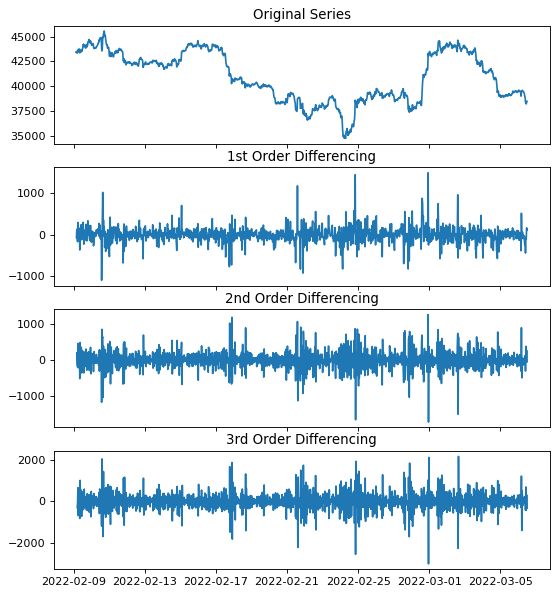
\includegraphics[width=0.495\textwidth]{./plots/arima/plots_btc/btc_30m_diff}}
  \subfloat[Autocorrelograma]{
   \label{f:fac}
    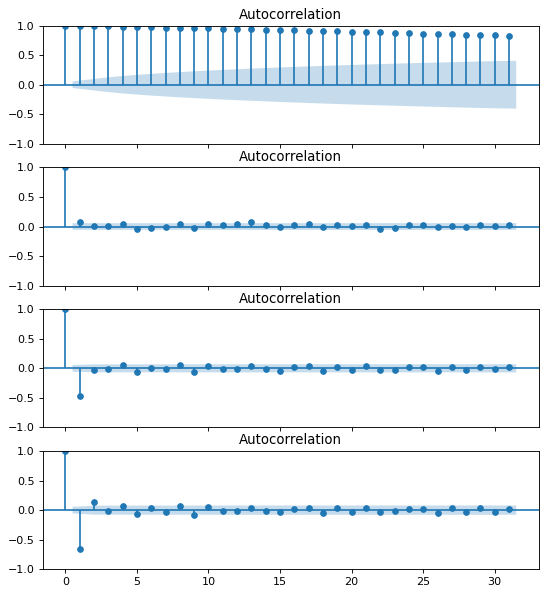
\includegraphics[width=0.48\textwidth]{./plots/arima/plots_btc/btc_30m_fac}}
  \caption{Sucesivas diferenciaciones y efecto en el autocorrelograma para la serie temporal de BTC con periodo de 30 minutos.}
  \label{f:btc_30m_diff-fac}
\end{figure}


\begin{figure}[H]
 \centering
  \subfloat[Correlograma Parcial. $p=2$]{
   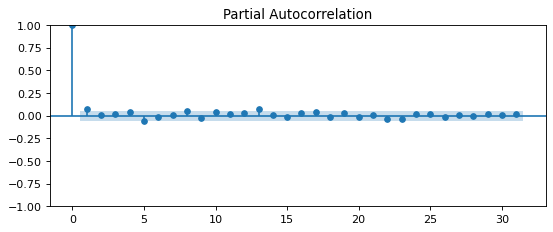
\includegraphics[width=0.5\textwidth]{./plots/arima/plots_btc/btc_30m_pac_p}}
  \subfloat[Correlograma $q=1$]{
   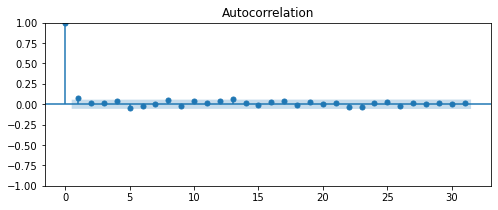
\includegraphics[width=0.5\textwidth]{./plots/arima/plots_btc/btc_30m_pac_q}}
  \caption{Diferenciación para el parámetro $p$ y $q$}
  \label{f:fac_btc_30m}
\end{figure}

\begin{figure}[H]
 \centering
  \subfloat[Diferenciaciones]{
   \label{f:diff}
    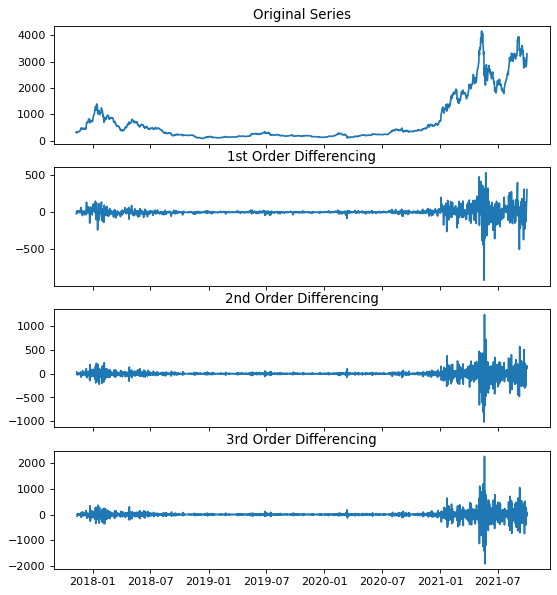
\includegraphics[width=0.495\textwidth]{./plots/arima/plots_eth/eth_1d_diff}}
  \subfloat[Autocorrelograma]{
   \label{f:fac}
    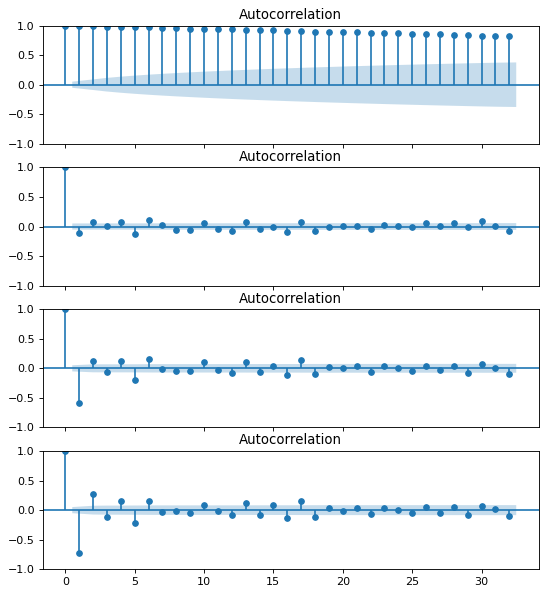
\includegraphics[width=0.48\textwidth]{./plots/arima/plots_eth/eth_1d_fac}}
  \caption{Sucesivas diferenciaciones y efecto en el autocorrelograma para la serie temporal de ETH con periodo de 1 día.}
  \label{f:eth_1d_diff-fac}
\end{figure}

\begin{figure}[H]
 \centering
  \subfloat[Correlograma Parcial. $p=2$]{
   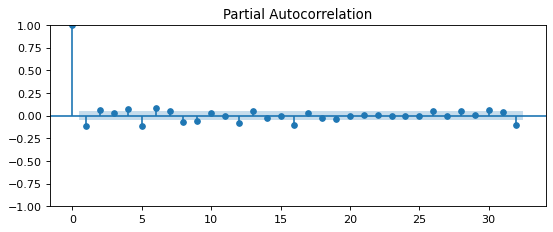
\includegraphics[width=0.5\textwidth]{./plots/arima/plots_eth/eth_1d_pac_p}}
  \subfloat[Correlograma $q=1$]{
   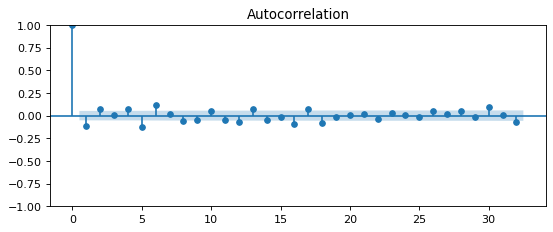
\includegraphics[width=0.5\textwidth]{./plots/arima/plots_eth/eth_1d_pac_q}}
  \caption{Diferenciación para el parámetro $p$ y $q$}
  \label{f:fac_eth_1d}
\end{figure}

\begin{figure}[H]
 \centering
  \subfloat[Diferenciaciones]{
   \label{f:diff}
    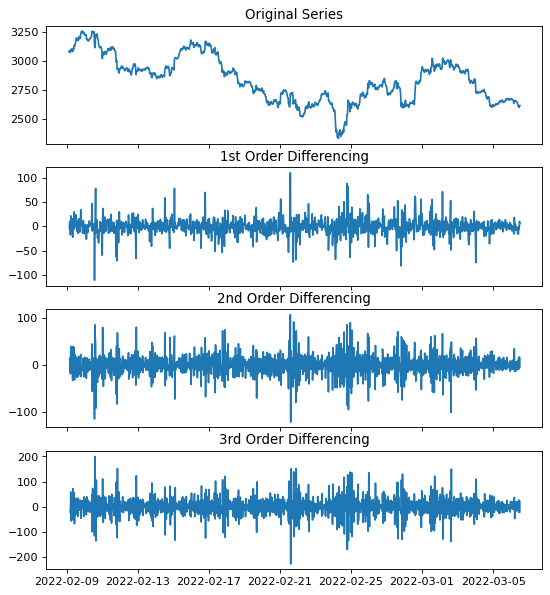
\includegraphics[width=0.48\textwidth]{./plots/arima/plots_eth/eth_30m_diff}}
  \subfloat[Autocorrelograma]{
   \label{f:fac}
    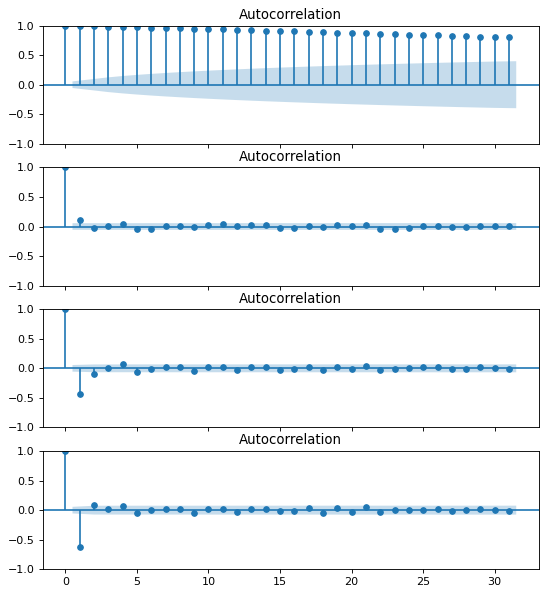
\includegraphics[width=0.48\textwidth]{./plots/arima/plots_eth/eth_30m_fac}}
  \caption{Sucesivas diferenciaciones y efecto en el autocorrelograma para la serie temporal de ETH con periodo de 30 minutos.}
  \label{f:eth_30m_diff-fac}
\end{figure}

\begin{figure}[H]
 \centering
  \subfloat[Correlograma Parcial. $p=2$]{
   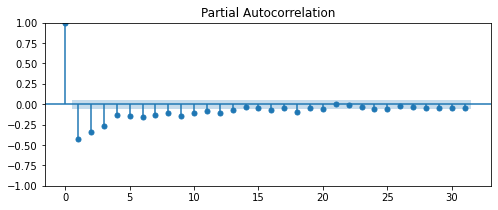
\includegraphics[width=0.5\textwidth]{./plots/arima/plots_eth/eth_30m_pac_p}}
  \subfloat[Correlograma $q=1$]{
   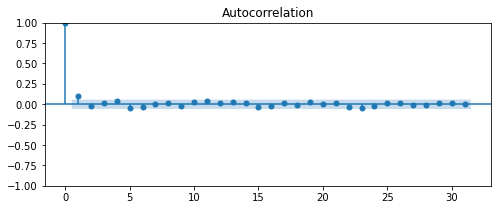
\includegraphics[width=0.5\textwidth]{./plots/arima/plots_eth/eth_30m_pac_q}}
  \caption{Diferenciación para el parámetro $p$ y $q$}
  \label{f:fac_eth_30m}
\end{figure}

\begin{figure}[H]
 \centering
  \subfloat[Diferenciaciones]{
   \label{f:diff}
    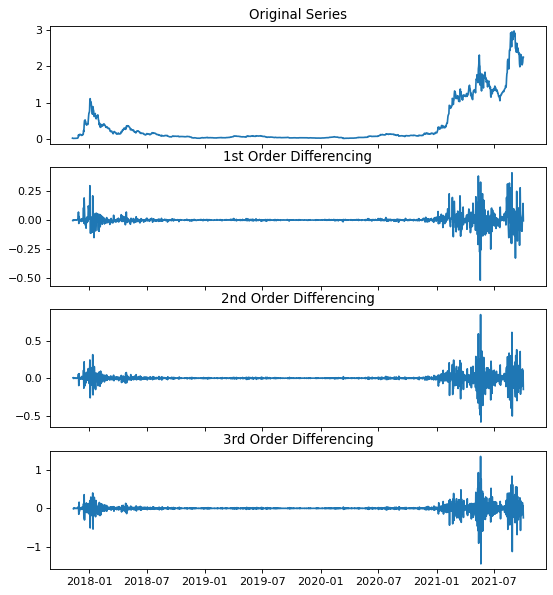
\includegraphics[width=0.48\textwidth]{./plots/arima/plots_ada/ada_1d_diff}}
  \subfloat[Autocorrelograma]{
   \label{f:fac}
    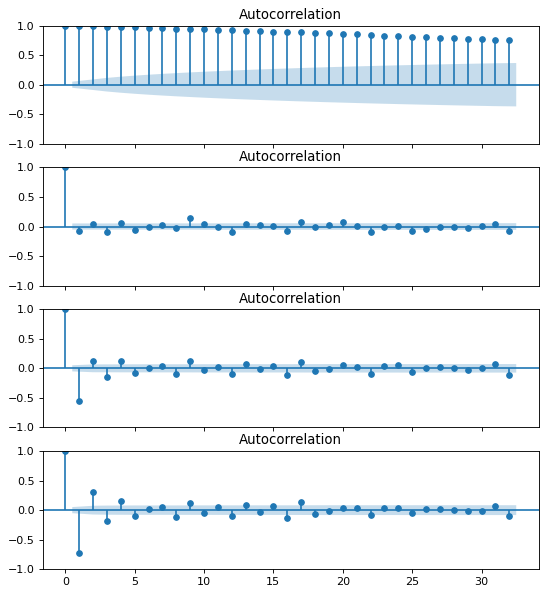
\includegraphics[width=0.48\textwidth]{./plots/arima/plots_ada/ada_1d_fac}}
  \caption{Sucesivas diferenciaciones y efecto en el autocorrelograma para la serie temporal de ADA con periodo de 1 día.}
  \label{f:ada_1d_diff-fac}
\end{figure}

\begin{figure}[H]
 \centering
  \subfloat[Correlograma Parcial. $p=2$]{
   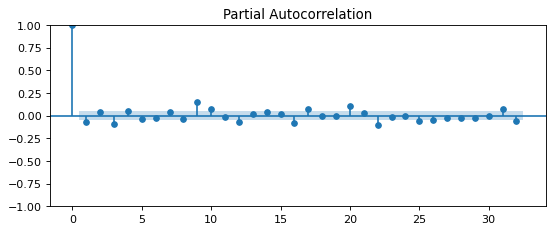
\includegraphics[width=0.5\textwidth]{./plots/arima/plots_ada/ada_1d_pac_p}}
  \subfloat[Correlograma $q=1$]{
   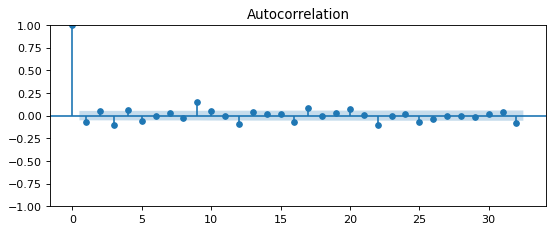
\includegraphics[width=0.5\textwidth]{./plots/arima/plots_ada/ada_1d_pac_q}}
  \caption{Diferenciación para el parámetro $p$ y $q$}
  \label{f:fac_ada_1d}
\end{figure}

\begin{figure}[H]
 \centering
  \subfloat[Diferenciaciones]{
   \label{f:diff}
    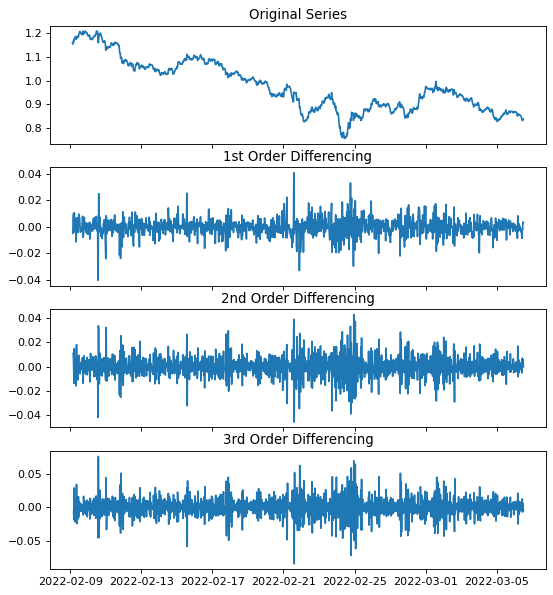
\includegraphics[width=0.48\textwidth]{./plots/arima/plots_ada/ada_30m_diff}}
  \subfloat[Autocorrelograma]{
   \label{f:fac}
    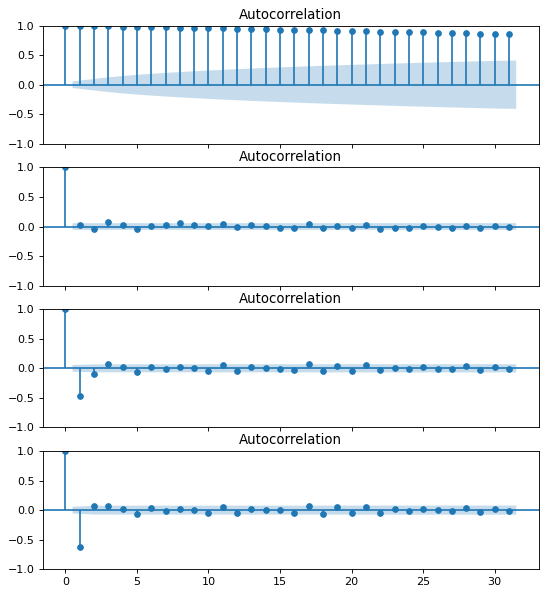
\includegraphics[width=0.48\textwidth]{./plots/arima/plots_ada/ada_30m_fac}}
  \caption{Sucesivas diferenciaciones y efecto en el autocorrelograma para la serie temporal de ADA con periodo de 30 minutos.}
  \label{f:ada_30m_diff-fac}
\end{figure}

\begin{figure}[H]
 \centering
  \subfloat[Correlograma Parcial. $p=2$]{
   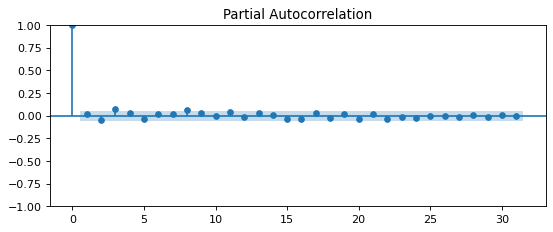
\includegraphics[width=0.5\textwidth]{./plots/arima/plots_ada/ada_30m_pac_p}}
  \subfloat[Correlograma $q=1$]{
   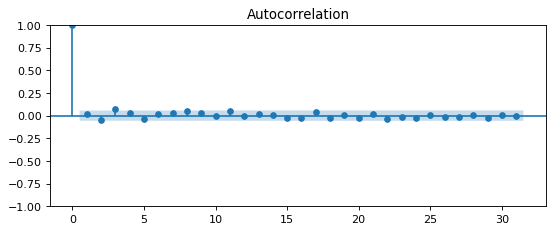
\includegraphics[width=0.5\textwidth]{./plots/arima/plots_ada/ada_30m_pac_q}}
  \caption{Diferenciación para el parámetro $p$ y $q$}
  \label{f:fac_ada_30m}
\end{figure}

\end{document}
